%-----------------------------------------------------------
% These packages are essential to produce the poster
%-----------------------------------------------------------
\usepackage[scale=1.24]{beamerposter}
\usepackage{graphicx,amsfonts}
\usepackage{pdfpages}
\newcounter{figura}
\setcounter{figura}{1}

%-----------------------------------------------------------
% Custom commands that I use frequently
%-----------------------------------------------------------
\newcommand{\bb}[1]{\mathbb{#1}}
\newcommand{\cl}[1]{\mathcal{#1}}
\newcommand{\fA}{\mathfrak{A}}
\newcommand{\fB}{\mathfrak{B}}
\newcommand{\Tr}{{\rm Tr}}
\newtheorem{thm}{Theorem}
\newcommand{\captione}[2]{\begin{minipage}[l]{#1}\begin{center} \textit{Figure \thefigura.}\  #2\end{center}\end{minipage}\addtocounter{figura}{1}}
\newcommand{\spacer}{\begin{column}{\sepwid}\end{column}}
\newcommand{\toplogo}[2]{\newcommand{\posterlogo}{\includegraphics[width=#1]{mypics/#2}}}
\newcommand{\extrainfo}[1]{\newcommand{\inforight}{#1}}
\newcommand{\moreinfo}[1]{\newcommand{\inforightother}{#1}}
\newcommand{\conjetura}[2]{\\[-8mm]\begin{minipage}[l]{45cm}\emph{#1}\end{minipage}& \,\hspace{2cm} \emph{#2}\hspace{2cm}\,\\[-6mm]  \\ \hline}


%-------------------------------------------------------------------------------------------------------------------------------
% These commands will help me to build new blocks, do not modify!
%-------------------------------------------------------------------------------------------------------------------------------

\def\newblock#1#2#3{\expandafter\def\csname Block#1\endcsname{\begin{block}{#2}\rmfamily{#3}\end{block}}}
\def\newAlert#1#2#3{\expandafter\def\csname Alert#1\endcsname{\begin{alertblock}{#2}\rmfamily{#3}\end{alertblock}}}
\def\newSingle#1#2{\expandafter\def\csname Single#1\endcsname{\begin{column}{\onecolwid}#2\end{column}}}
\def\newMarried#1#2{\expandafter\def\csname Married#1\endcsname{\begin{column}{\twocolwid}#2\end{column}}}
\def\newTwin#1#2{\expandafter\def\csname Twin#1\endcsname{\begin{columns}[t,totalwidth=\twocolwid]#2\end{columns}}}





%-----------------------------------------------------------
% Define the column width and poster size
% To set effective sepwid, onecolwid and twocolwid values, first choose how many columns you want and how much separation you want between columns
% The separation I chose is 0.024 and I want 4 columns
% Then set onecolwid to be (1-(4+1)*0.024)/4 = 0.22
% Set twocolwid to be 2*onecolwid + sepwid = 0.464
%-----------------------------------------------------------

\newlength{\sepwid}
\newlength{\onecolwid}
\newlength{\twocolwid}
\setlength{\paperwidth}{48in}
\setlength{\paperheight}{36in}
\setlength{\sepwid}{0.024\paperwidth}
\setlength{\onecolwid}{0.22\paperwidth}
\setlength{\twocolwid}{0.464\paperwidth}
\setlength{\topmargin}{-0.5in}
\usetheme{confposter}

%-----------------------------------------------------------
% Define colours (see beamerthemeconfposter.sty to change these colour definitions)
%-----------------------------------------------------------

\setbeamercolor{block title}{fg=ngreen,bg=white}
\setbeamercolor{block body}{fg=black,bg=white}
\setbeamercolor{block alerted title}{fg=white,bg=dblue!70}
\setbeamercolor{block alerted body}{fg=black,bg=dblue!10}






%-----------------------------------------------------------------------------------------------------------------------------------------
%                               START TYPING YOUR BLOCKS !!
%-----------------------------------------------------------------------------------------------------------------------------------------
%%%%%%%%%%%%%%%%%%%%%%%%%%%%%%%%%%%%%%%%%%%%%  IMPORTANT %%%%%%%%%%%%%%%%%%%%%%%%%%%%%%%%%%%%%%%%%%%%%%%%%%%%%%%%%%%%%%%%%%%%%%%%%%%%%%%%%
%%%%%%%%%%%%%%%%%%%%%%%%%%%%%%%%%%%%%%%%%%%%%  IMPORTANT %%%%%%%%%%%%%%%%%%%%%%%%%%%%%%%%%%%%%%%%%%%%%%%%%%%%%%%%%%%%%%%%%%%%%%%%%%%%%%%%%
%%%   NO EMPTY ROWS. This example shows what you are NOT to do:
%%%  \newAlert{Main}{Main First Example}{
%%%             This is the main topic, blah blah blah
%%%
%%%             and then blah blah blah
%%%             }
%%%%%%%%%%%%%%%%%%%%%%%%%%%%%%%%%%%%%%%%%%%%%%%%%%%%%%%%%%%%%%%%%%%%%%%%%%%%%%%%%%%%%%%%%%%%%%%%%%%%%%%%%%%%%%%%%%%%%%%%%%%%%%%%%%%%%%%%%%
















%%%%%%%%%%%%%%%%%%%%%%%%%%%%%%%%%%%%%%%%%%%%%%%%%%%%%%%%%%%%%%%%%%%%%%%%%%%%%%%%%%%%%%%%%%%%%%%%%%%%%%%%%%%%%%%%%%%%%%%%%%%%%%%%%%%%%%%%%%%
%%%%%%%%%%%%%%%%%%%%%%%%%%%%%%%%%%%%%%%%%%%%%%%%%%%%%%%%%%%%%%%%%%%%%%%%%%%%%%%%%%%%%%%%%%%%%%%%%%%%%%%%%%%%%%%%%%%%%%%%%%%%%%%%%%%%%%%%%%%
%%%%%%%%%%%%%%%%%%%%%%%%%%%%%%%%%%%%%%%%%%%%             REGULAR    BLOCKS  START          %%%%%%%%%%%%%%%%%%%%%%%%%%%%%%%%%%%%%%%%%%%%%%%%
%%%%%%%%%%%%%%%%%%%%%%%%%%%%%%%%%%%%%%%%%%%%%%%%%%%%%%%%%%%%%%%%%%%%%%%%%%%%%%%%%%%%%%%%%%%%%%%%%%%%%%%%%%%%%%%%%%%%%%%%%%%%%%%%%%%%%%%%%%%
%%%%%%%%%%%%%%%%%%%%%%%%%%%%%%%%%%%%%%%%%%%%%%%%%%%%%%%%%%%%%%%%%%%%%%%%%%%%%%%%%%%%%%%%%%%%%%%%%%%%%%%%%%%%%%%%%%%%%%%%%%%%%%%%%%%%%%%%%%%




%%%%%%%%%%%%%%%%%%%%%%%%%%%%%%%%%%%%%%%%%%%%%%%%%%%%%%%%%%%%%%%%%%%%%%%%%%%%%%%%%%%%%%%%%%%%%%%%%%%%%%%%%%%%%%%%%%%%%%%%%%%%%%%%%%%%%%%%%%%
\newblock{Introduction}{Introduction}{
        The purpose of our research is to study distributed search-and-escape algorithms.
        These algorithms involve mobile agents (or robots) searching in geometric domains, such as a closed disk or a convex polygon.
        By working together and communicating with one another, the mobile agents search for an exit hidden on the perimeter.
        The goal of our research is to create and study exit strategies that terminate as quickly as possible.
        }
%%%%%%%%%%%%%%%%%%%%%%%%%%%%%%%%%%%%%%%%%%%%%%%%%%%%%%%%%%%%%%%%%%%%%%%%%%%%%%%%%%%%%%%%%%%%%%%%%%%%%%%%%%%%%%%%%%%%%%%%%%%%%%%%%%%%%%%%%%%








%%%%%%%%%%%%%%%%%%%%%%%%%%%%%%%%%%%%%%%%%%%%%%%%%%%%%%%%%%%%%%%%%%%%%%%%%%%%%%%%%%%%%%%%%%%%%%%%%%%%%%%%%%%%%%%%%%%%%%%%%%%%%%%%%%%%%%%%%%%
\newblock{Definitions}{Definitions}{
         \begin{description}[font=$\bullet$~\normalfont\textbf]
             \item[$\bullet$ An exit] is a point unknown to the agents, that is located on an perimeter on the domain. The agents must find the exit for the algorithm to finish.
             \item[$\bullet$ A priority] agent is one that must reach the exit for the algorithm to terminate.
             \item[$\bullet$ A helper]   agent is one that simply assists the priority agent(s) in finding the exit.
             \item[$\bullet$ Algorithm termination] occurs if a specified subset of agents shares a position with the exit.
         \end{description}
         }
%%%%%%%%%%%%%%%%%%%%%%%%%%%%%%%%%%%%%%%%%%%%%%%%%%%%%%%%%%%%%%%%%%%%%%%%%%%%%%%%%%%%%%%%%%%%%%%%%%%%%%%%%%%%%%%%%%%%%%%%%%%%%%%%%%%%%%%%%%%








%%%%%%%%%%%%%%%%%%%%%%%%%%%%%%%%%%%%%%%%%%%%%%%%%%%%%%%%%%%%%%%%%%%%%%%%%%%%%%%%%%%%%%%%%%%%%%%%%%%%%%%%%%%%%%%%%%%%%%%%%%%%%%%%%%%%%%%%%%%
\newblock{Description}{Algorithm Description}{
         In our algorithm, we use two \textbf{priority} agents and one \textbf{helper} agent.
         The termination condition in our algorithm is reached when either one of the two priority agents reaches the exit.
         % INCLUDE A FRAME OF REFERENCE. 0 DEGREES IS AT 3:00. %
         We send one priority and one helper to some angle $\alpha$ on the perimeter of the shape, in the third quadrant.
         The priority agent travels counter-clockwise, and the helper travels clockwise.
         The other priority agent travels to 0 radians and travels counter-clockwise.
         % INCLUDE A FRAME OF REFERENCE. 0 DEGREES IS AT 3:00. %
         }

 \newblock{DescriptionDos}{Algorithm Description (Cont)}{
          We may compare this method of sending two agents out together and separating them
          with a more naive method of sending the agents out at equal distances. If we were
          to send all agents out at an angle of $\ 2 \pi / 3$ and having them all travel
          in the same direction, we see that in the worst case, the helper will find the exit
          and the very end of its searched area and both agents will be equally close to it.
          This will result in a time of \textbf{$1 + 2 \pi /3 + 2 \sin \pi / 3$}, or \textbf{4.826 time units.}
          This is significantly longer than our solution of \textbf{3.55 time units}.
          }
%%%%%%%%%%%%%%%%%%%%%%%%%%%%%%%%%%%%%%%%%%%%%%%%%%%%%%%%%%%%%%%%%%%%%%%%%%%%%%%%%%%%%%%%%%%%%%%%%%%%%%%%%%%%%%%%%%%%%%%%%%%%%%%%%%%%%%%%%%%

%	the exit is unknown, and that this is an animation of a distributed algorithm,
%	and in the is distibuted algoirithm, we have a multiple bots trying to find an  exit,
%	where two are distinguished and one is a helper, where only one distinguish must reach.
%	crab.rutgers.edu/~shende/ rutgers library system first and search for them, or look through articles, by a link that says do you want an onlune version, which will give access to al l the source, as in the pdf, but not directly.
%	2018 God save the queen
%	fun with algorithms - god saves the queen
%




%%%%%%%%%%%%%%%%%%%%%%%%%%%%%%%%%%%%%%%%%%%%%%%%%%%%%%%%%%%%%%%%%%%%%%%%%%%%%%%%%%%%%%%%%%%%%%%%%%%%%%%%%%%%%%%%%%%%%%%%%%%%%%%%%%%%%%%%%%%
\newblock{Work}{Future Work}{
	    Later on we will study further distributed algorithms of search and escape, such as lines or triangles.
        }
%%%%%%%%%%%%%%%%%%%%%%%%%%%%%%%%%%%%%%%%%%%%%%%%%%%%%%%%%%%%%%%%%%%%%%%%%%%%%%%%%%%%%%%%%%%%%%%%%%%%%%%%%%%%%%%%%%%%%%%%%%%%%%%%%%%%%%%%%%%










%%%%%%%%%%%%%%%%%%%%%%%%%%%%%%%%%%%%%%%%%%%%%%%%%%%%%%%%%%%%%%%%%%%%%%%%%%%%%%%%%%%%%%%%%%%%%%%%%%%%%%%%%%%%%%%%%%%%%%%%%%%%%%%%%%%%%%%%%%%
\newblock{Conclusions}{Conclusions}{
	This algorithm has an upper bound of 3.55 time units, being faster than an algorithm of one distinguished and two helpers with an upper bound of 3.83 time units. We can achieve this time by sending our Helper and Distinguished agents out at an angle of ($\pi + 5 \pi / 9 - 2\sqrt3$), so that
    both of the worst case time predictions are equal.
    This algorithm and many other like it have real world applications, such as
    having robots or drones be able to search for a safe exit in a room to evacuate humans in the event
    a disaster. By using this algorithm we can for example, quickly evacuate 1 of 2 doctors from an area
    in order to be able to get medical help to others as quickly as possible.
       }
%%%%%%%%%%%%%%%%%%%%%%%%%%%%%%%%%%%%%%%%%%%%%%%%%%%%%%%%%%%%%%%%%%%%%%%%%%%%%%%%%%%%%%%%%%%%%%%%%%%%%%%%%%%%%%%%%%%%%%%%%%%%%%%%%%%%%%%%%%%

















%%%%%%%%%%%%%%%%%%%%%%%%%%%%%%%%%%%%%%%%%%%%%%%%%%%%%%%%%%%%%%%%%%%%%%%%%%%%%%%%%%%%%%%%%%%%%%%%%%%%%%%%%%%%%%%%%%%%%%%%%%%%%%%%%%%%%%%%%%%
\newblock{Bibliography}{References}{\small
      \begin{thebibliography}{99}
         \bibitem{} Jurek Czyzowicz et al. (2014). Evacuating Robots via Unknown Exit in a Disk. Proceesings of DISC 2014, LNCS 8784, pp. 122-136, 2014.
         \bibitem{} Jurek Czyzowicz et al. (2015). Evacuating Robots From a Disk Using Face-To-Face Communication. Proceesings of CIAC, 2015 p. 140-152, 2015.
         \bibitem{} Jurek Czyzowicz, et. al., Priority Evacuation from a Disk Using Mobile Robots, Proceedings of SIROCCO, pages 392-407, 2018.
         \bibitem{} Jurek Czyzowicz, et. al., God Save the Queen. Fun with Algorithms, arXiv:1804.06011v1 [cs.MA] 17 Apr 2018.
      \end{thebibliography}
      }
%%%%%%%%%%%%%%%%%%%%%%%%%%%%%%%%%%%%%%%%%%%%%%%%%%%%%%%%%%%%%%%%%%%%%%%%%%%%%%%%%%%%%%%%%%%%%%%%%%%%%%%%%%%%%%%%%%%%%%%%%%%%%%%%%%%%%%%%%%%













%%%%%%%%%%%%%%%%%%%%%%%%%%%%%%%%%%%%%%%%%%%%%%%%%%%%%%%%%%%%%%%%%%%%%%%%%%%%%%%%%%%%%%%%%%%%%%%%%%%%%%%%%%%%%%%%%%%%%%%%%%%%%%%%%%%%%%%%%%%
\newblock{Acknowledgements}{Acknowledgements}{\small
      This research is supported by the National Science Foundation under grant \# CCf-AF 1813940 (RUI: Search, Evacuation and Reconfiguration with Coordinated Mobile Agents).
      }
%%%%%%%%%%%%%%%%%%%%%%%%%%%%%%%%%%%%%%%%%%%%%%%%%%%%%%%%%%%%%%%%%%%%%%%%%%%%%%%%%%%%%%%%%%%%%%%%%%%%%%%%%%%%%%%%%%%%%%%%%%%%%%%%%%%%%%%%%%%










%%%%%%%%%%%%%%%%%%%%%%%%%%%%%%%%%%%%%%%%%%%%%%%%%%%%%%%%%%%%%%%%%%%%%%%%%%%%%%%%%%%%%%%%%%%%%%%%%%%%%%%%%%%%%%%%%%%%%%%%%%%%%%%%%%%%%%%%%%%
\newblock{Logo}{}{\vspace{-4cm}
      \begin{center}
          
\includegraphics[width=1.5in]{mypics/temp.jpg}
      \end{center}
      }
%%%%%%%%%%%%%%%%%%%%%%%%%%%%%%%%%%%%%%%%%%%%%%%%%%%%%%%%%%%%%%%%%%%%%%%%%%%%%%%%%%%%%%%%%%%%%%%%%%%%%%%%%%%%%%%%%%%%%%%%%%%%%%%%%%%%%%%%%%%










%%%%%%%%%%%%%%%%%%%%%%%%%%%%%%%%%%%%%%%%%%%%%%%%%%%%%%%%%%%%%%%%%%%%%%%%%%%%%%%%%%%%%%%%%%%%%%%%%%%%%%%%%%%%%%%%%%%%%%%%%%%%%%%%%%%%%%%%%%%
%%%%%%%%%%%%%%%%%%%%%%%%%%%%%%%%%%%          REGULAR   BLOCKS     FINISH                   %%%%%%%%%%%%%%%%%%%%%%%%%%%%%%%%%%%%%%%%%%%%%%%%
%%%%%%%%%%%%%%%%%%%%%%%%%%%%%%%%%%%%%%%%%%%%%%%%%%%%%%%%%%%%%%%%%%%%%%%%%%%%%%%%%%%%%%%%%%%%%%%%%%%%%%%%%%%%%%%%%%%%%%%%%%%%%%%%%%%%%%%%%%%
















%%%%%%%%%%%%%%%%%%%%%%%%%%%%%%%%%%%%%%%%%%%%%%%%%%%%%%%%%%%%%%%%%%%%%%%%%%%%%%%%%%%%%%%%%%%%%%%%%%%%%%%%%%%%%%%%%%%%%%%%%%%%%%%%%%%%%%%%%%%
%%%%%%%%%%%%%%%%%%%%%%%%%%%%%%%%%%%%%%%%%%%%%%%%%%%%%%%%%%%%%%%%%%%%%%%%%%%%%%%%%%%%%%%%%%%%%%%%%%%%%%%%%%%%%%%%%%%%%%%%%%%%%%%%%%%%%%%%%%%
%%%%%%%%%%%%%%%%%%%%%%%%%%%%%%                  ALERT BLOCKS START                         %%%%%%%%%%%%%%%%%%%%%%%%%%%%%%%%%%%%%%%%%%%%%%%%
%%%%%%%%%%%%%%%%%%%%%%%%%%%%%%%%%%%%%%%%%%%%%%%%%%%%%%%%%%%%%%%%%%%%%%%%%%%%%%%%%%%%%%%%%%%%%%%%%%%%%%%%%%%%%%%%%%%%%%%%%%%%%%%%%%%%%%%%%%%
%%%%%%%%%%%%%%%%%%%%%%%%%%%%%%%%%%%%%%%%%%%%%%%%%%%%%%%%%%%%%%%%%%%%%%%%%%%%%%%%%%%%%%%%%%%%%%%%%%%%%%%%%%%%%%%%%%%%%%%%%%%%%%%%%%%%%%%%%%%


\newAlert{MainTopic}{Figures}{
                     \begin{center}
                         \begin{subfigure}
                             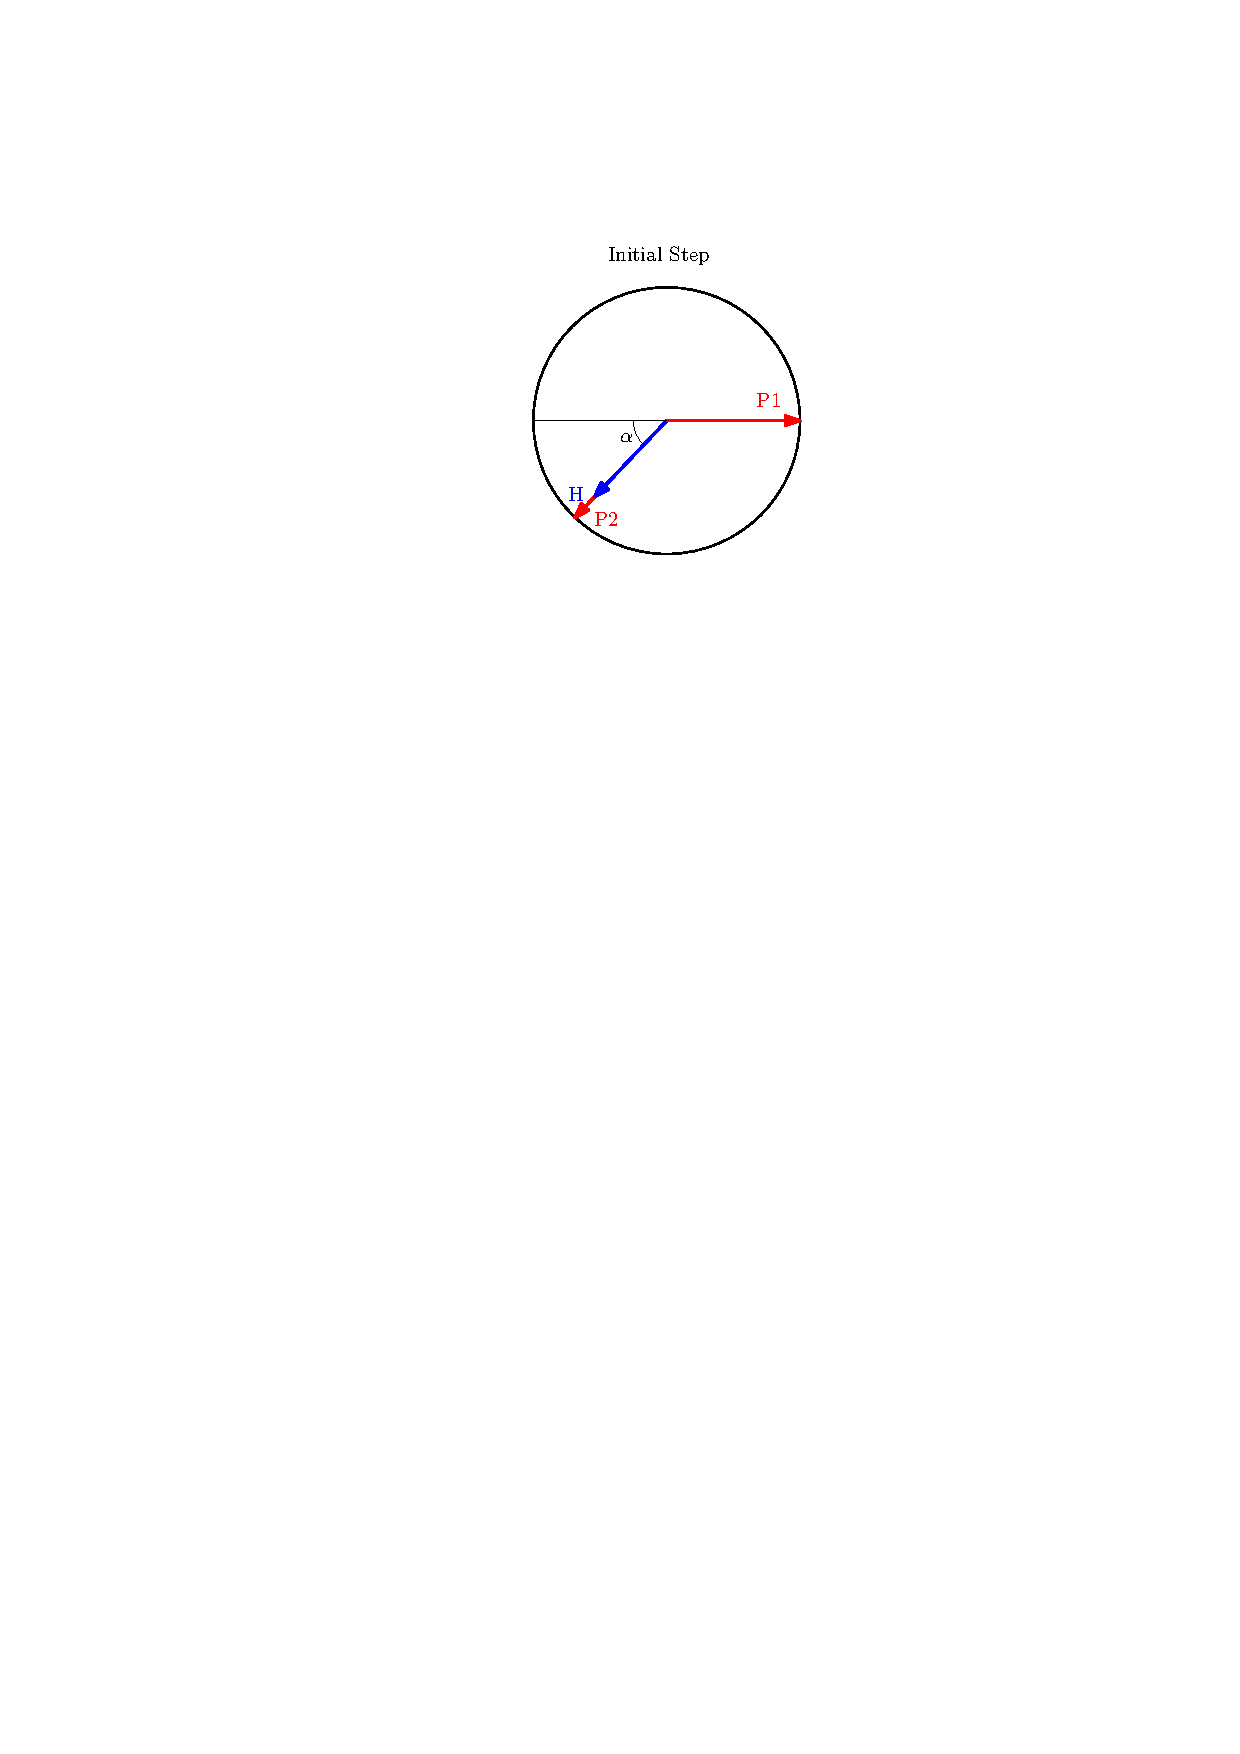
\includegraphics[width=0.23\textwidth]{mypics/2Q1S_Initial.pdf}
                         \end{subfigure}
                         \begin{subfigure}
                             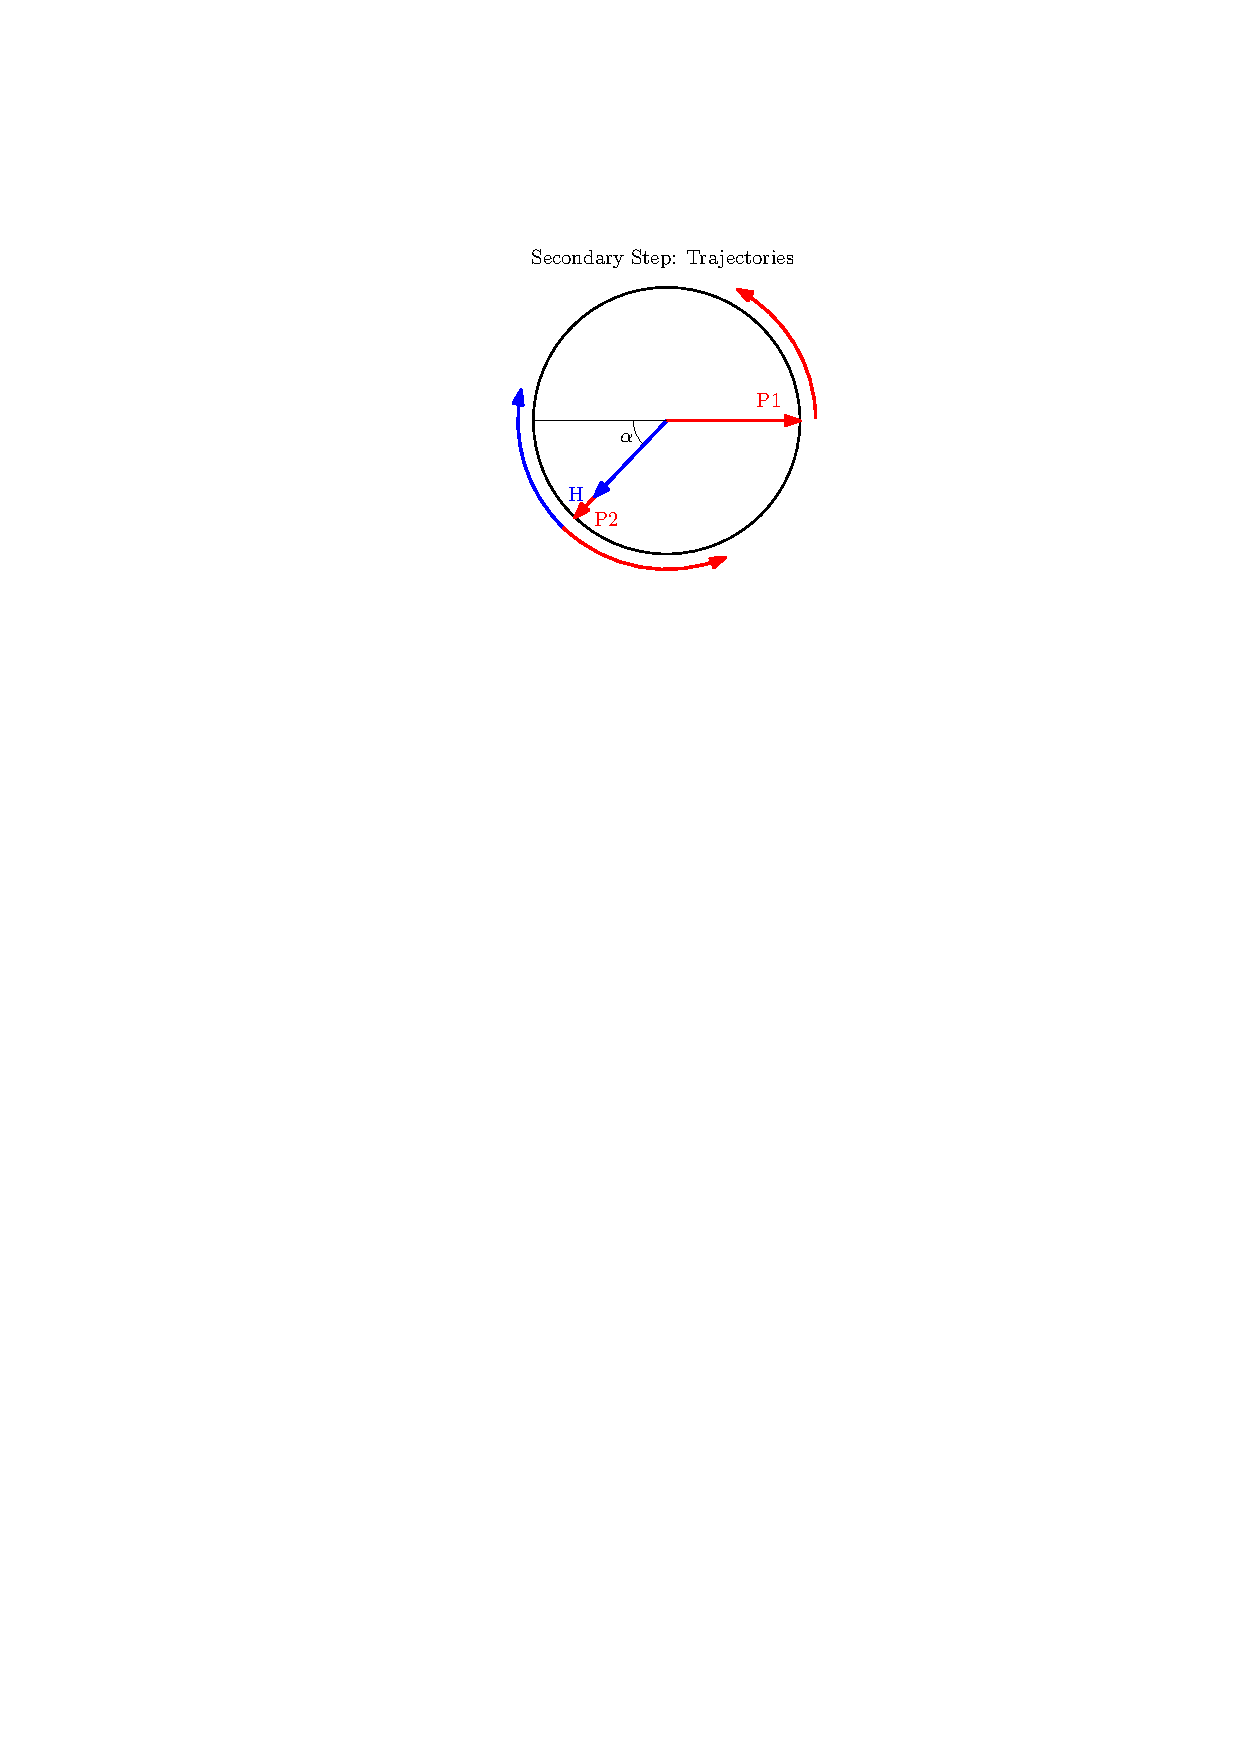
\includegraphics[width=0.2\textwidth]{mypics/2Q1S_Second_Step.pdf}
                         \end{subfigure}
                         \begin{subfigure}
                             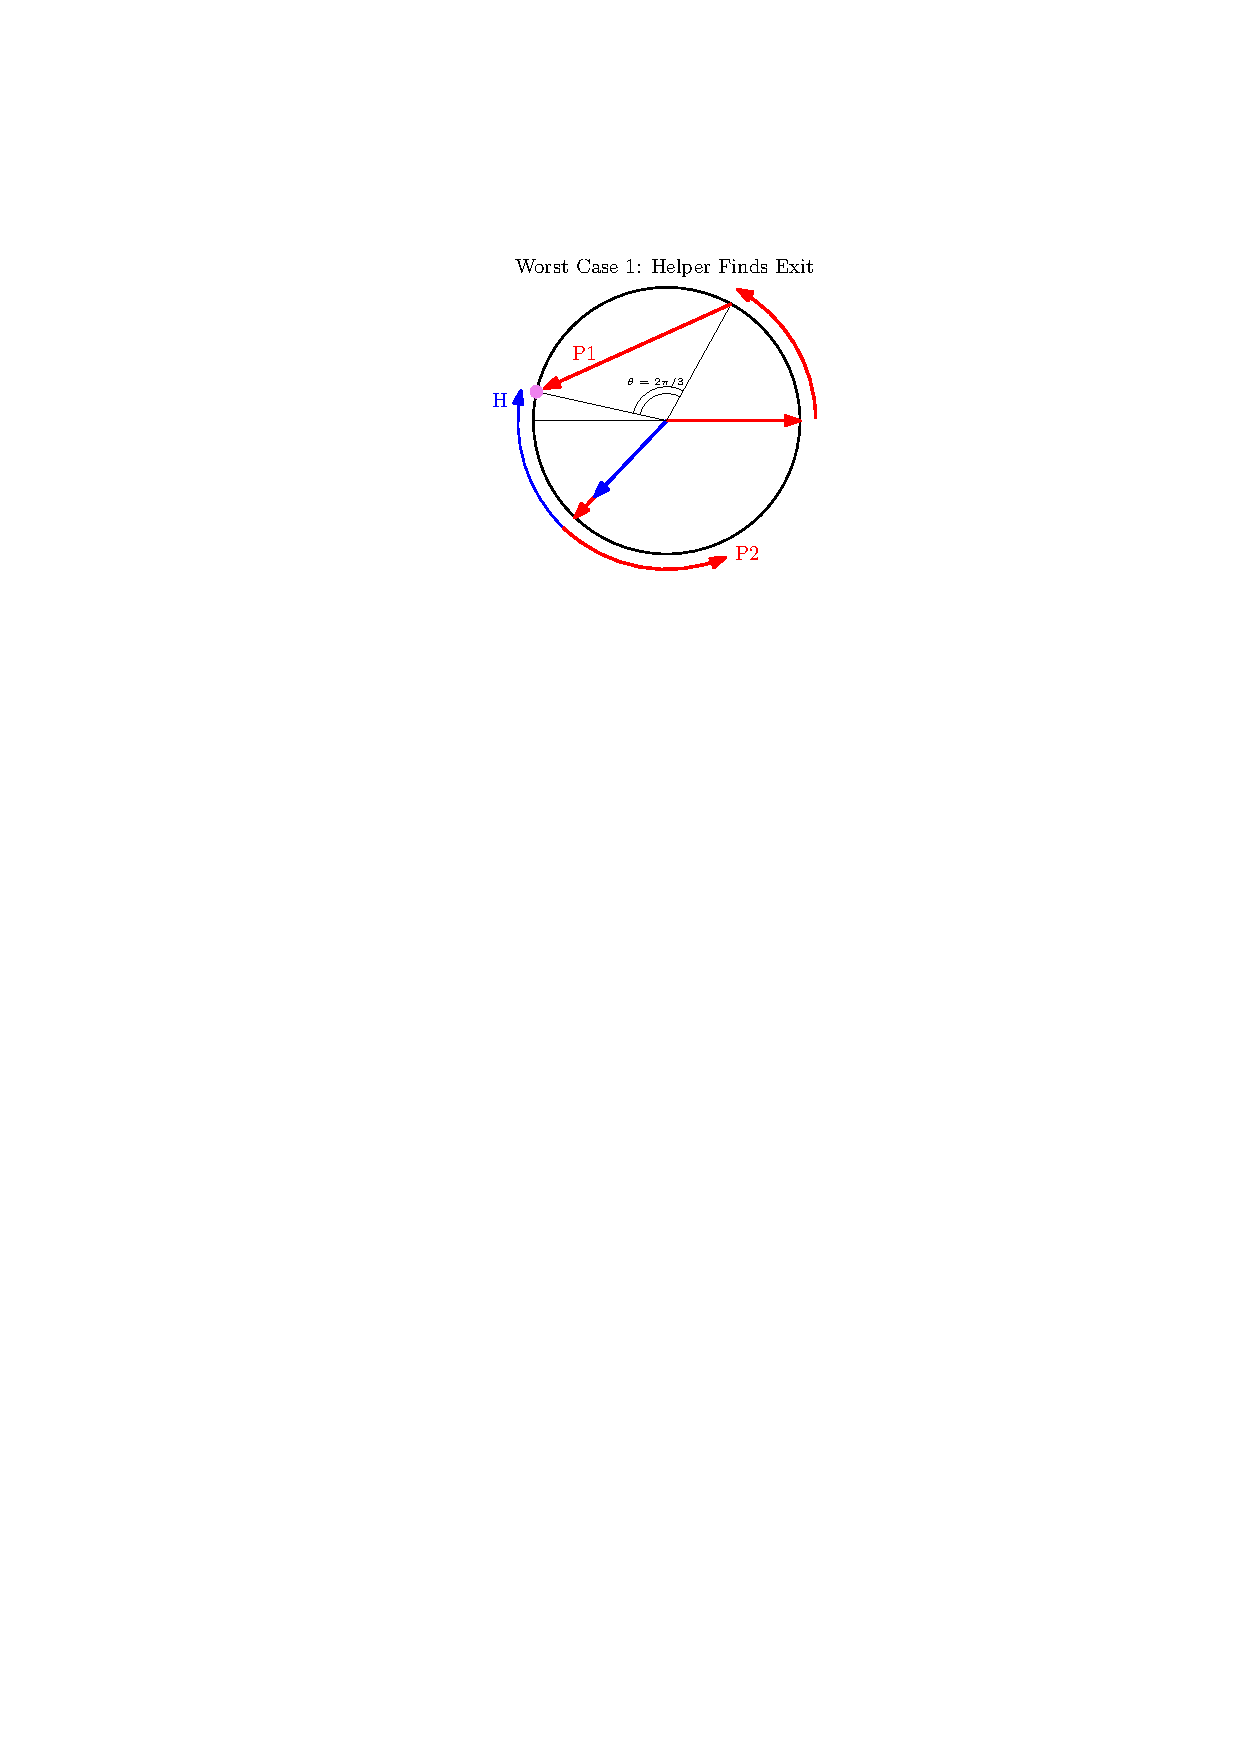
\includegraphics[width=0.22\textwidth]{mypics/2Q1S_WorstCase_Servant.pdf}
                         \end{subfigure}
                         \begin{subfigure}
                             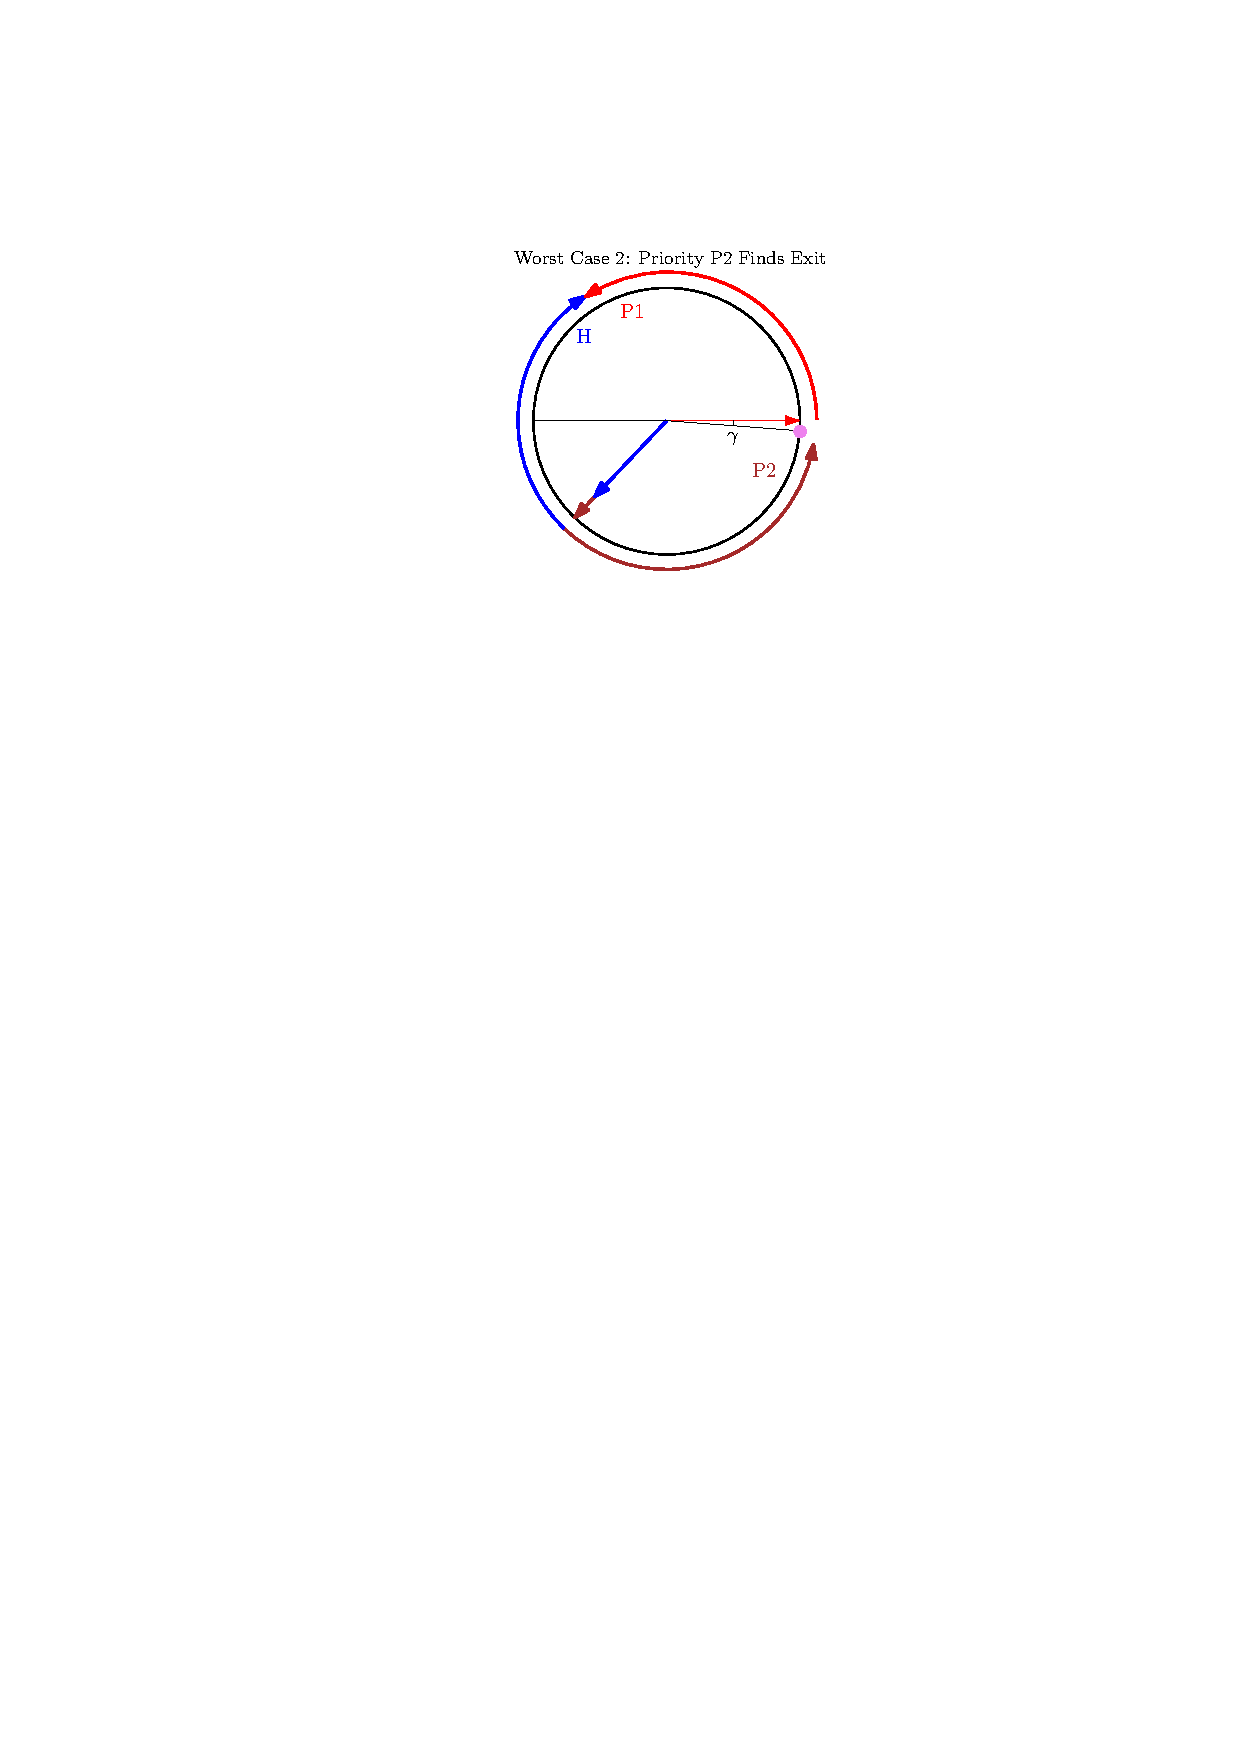
\includegraphics[width=0.2\textwidth]{mypics/2Q1S_WorstCase_Priority.pdf}
                         \end{subfigure}
%                         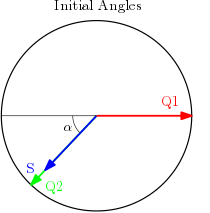
\includegraphics[width=3in]{mypics/2Q1S_Initial.png}\hspace{1cm}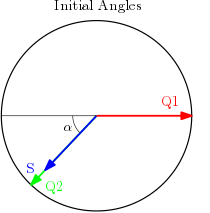
\includegraphics[width=3in]{mypics/2Q1S_Initial.png}\hspace{1cm}  \\[.2cm]
%                         \captione{3in}{Inital Steps}
%                         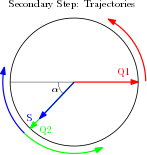
\includegraphics[width=3in]{mypics/2Q1S_Secondary.png}\hspace{1cm}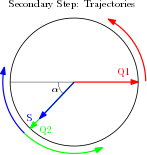
\includegraphics[width=3in]{mypics/2Q1S_Secondary.png}\hspace{1cm}  \\[.2cm]
%                         \captione{3in}{Secondary Step: Trajectories}
                    \end{center}
            }

\newAlert{MainProblem}{Main Result}{
            The purpose of our research is to propose an algorithm for two
            distinguished agents and a helper agent to find an unknown
            exit on a disk. We show that this can be achieved in no more than
            3.55 time units. This result does not represent all algorithms using
            3 agents, nor does it represent all algorithms using distinguished agents.
            \begin{center}
                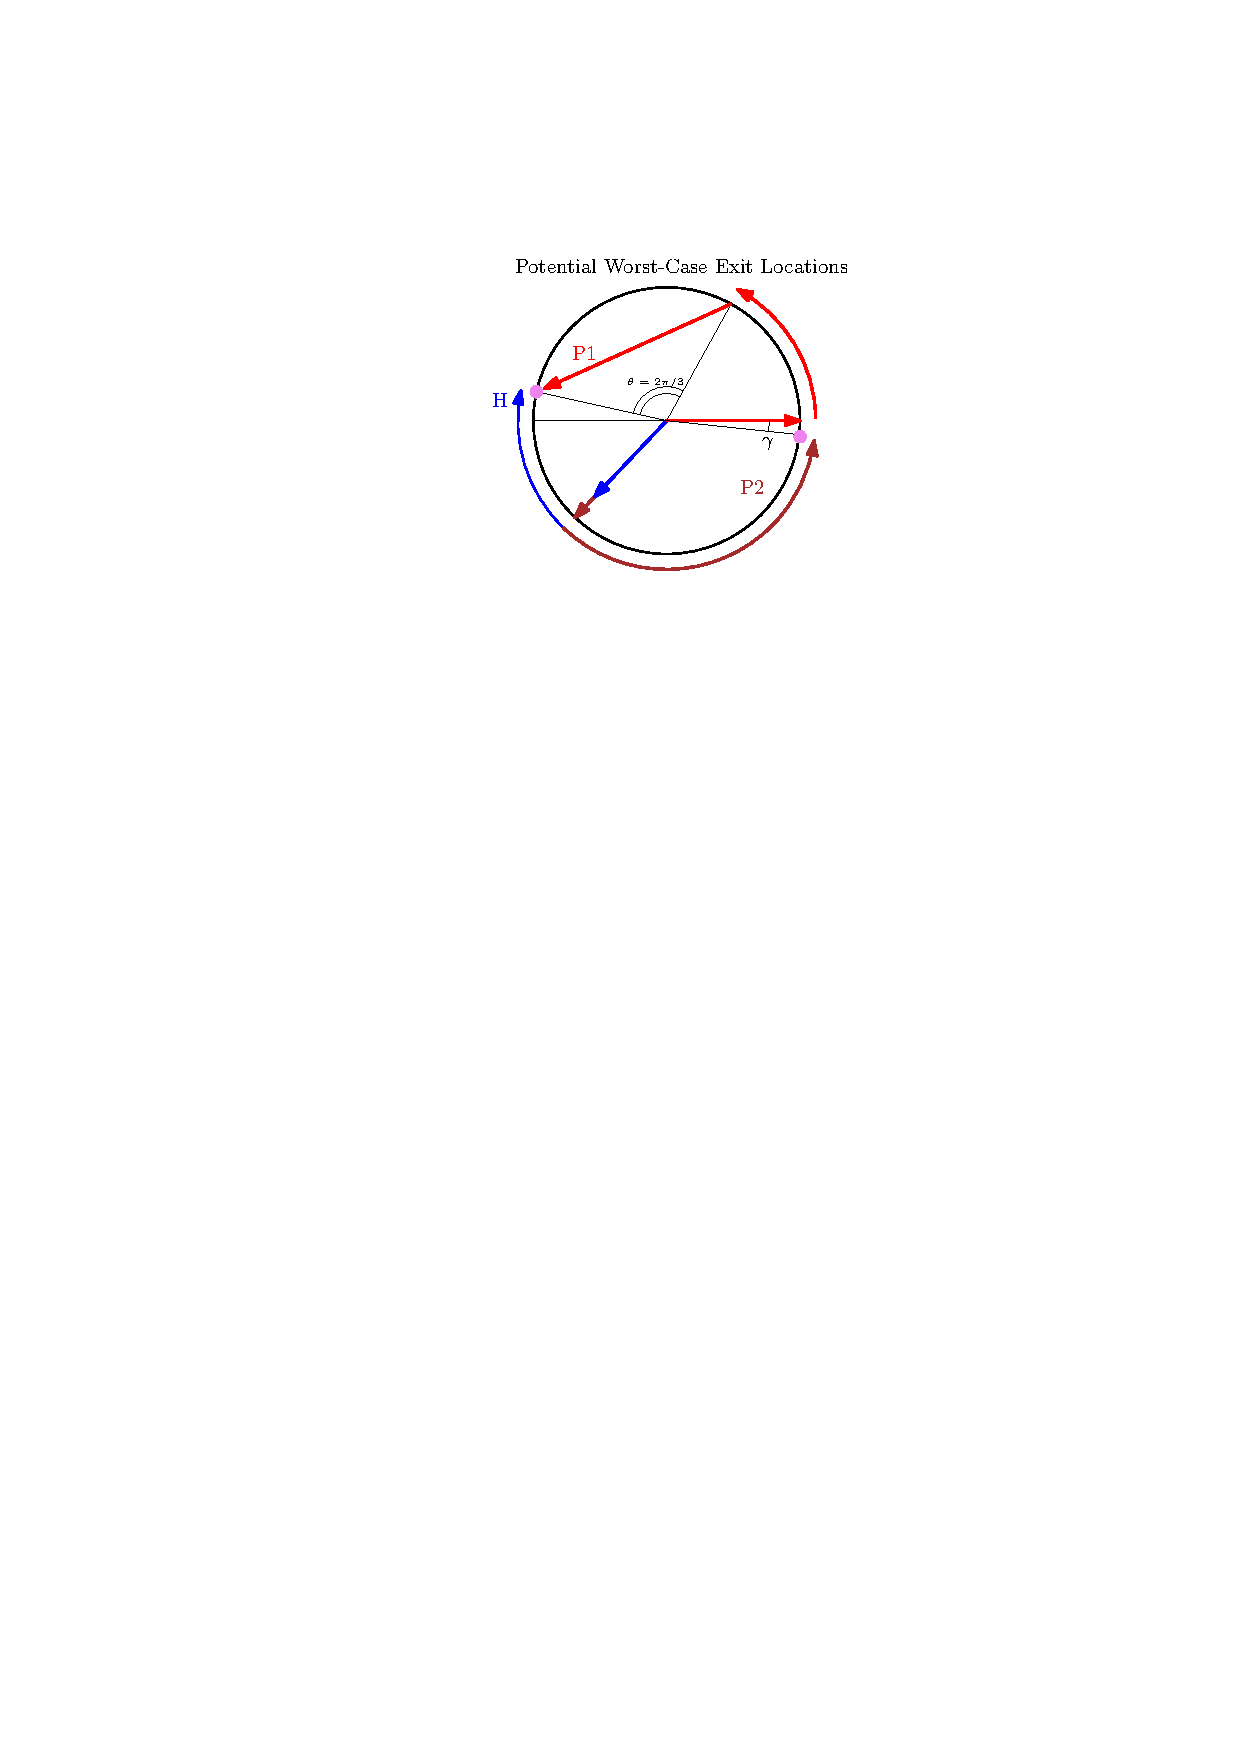
\includegraphics[width=0.6\textwidth]{mypics/2Q1S_WorstCase_Both.pdf}
            \end{center}
            }

\newAlert{Conjectures}{Our Conjectures and Analysis}{
            In this algorithm, we observe two worst case situations. In one, the priority
            robot assigned to the third and fourth quadrant travels the entire distance
            of its arc, until it reaches the exit a small distance before 0 radians (Fig. 3 above).
            In the other, the helper agent finds the exit at a point such that the closest priority
            agent would have to travel along a chord to reach it (Fig. 4 above).\vspace{0.5in}\hfill\break % MAKE A NEW LINE WITH A SPACE
            We analyze the case in which the helper agent finds the exit in the second quadrant.
            Say that there is an angle of $\theta$ between the closest priority and the helper agent, so that
            the shortest distance between the two agents is $\[ 2 \sin (\theta / 2)$ . The angle $\theta$ that
            would produce the longest distance between the priority agent along the top and the helper, is $\theta = 2 \pi / 3$.
            Therefore, the termination time for the algorithm in this case is $\[ 1 + \alpha + 2 \sin (\theta / 2)$, where $\alpha$ is the
            circumfrential distance already traveled by each robot. We can set this result equal to the termination time of the agent that explores the
            bottom part of the circle, which is $\[ 1 + \delta$, where $\delta$ is a distance traveled by the priority agent such that
            it finds the exit a small distance $\gamma$ before angle 0 (Fig. 4 Above.).
            \vfill
            }


%%%%%%%%%%%%%%%%%%%%%%%%%%%%%%%%%%%%%%%%%%%%%%%%%%%%%%%%%%%%%%%%%%%%%%%%%%%%%%%%%%%%%%%%%%%%%%%%%%%%%%%%%%%%%%%%%%%%%%%%%%%%%%%%%%%%%%%%%%%
%%%%%%%%%%%%%%%%%%%%%%%%%%%%%%%%%%%         ALERT BLOCKS  FINISH                           %%%%%%%%%%%%%%%%%%%%%%%%%%%%%%%%%%%%%%%%%%%%%%%%
%%%%%%%%%%%%%%%%%%%%%%%%%%%%%%%%%%%%%%%%%%%%%%%%%%%%%%%%%%%%%%%%%%%%%%%%%%%%%%%%%%%%%%%%%%%%%%%%%%%%%%%%%%%%%%%%%%%%%%%%%%%%%%%%%%%%%%%%%%%









%%%%%%%%%%%%%%%%%%%%%%%%%%%%%%%%%%%%%%%%%%%%%%   TIPS  TO MAKE A NICE POSTER  %%%%%%%%%%%%%%%%%%%%%%%%%%%%%%%%%%%%%%%%%%%%%%%%%%%%%%%%%%%%%
% Common mistakes when compiling
% 1) There is an empty row in one of the blocks, remove it.
% 2) You forgot to close the brace } at the end of the block, close it.
% 3) The name of a block does not agree, for example you have \newSingle{Description}{\BlockDescription}
%                           and when you call it to form the main columns, you may have typed \SingleDescripption
%                           hence you should have typed  \SingleDescription, correct it.
% 4) It can not find a picture, perhaps you have it in the wrong folder.
% 5) Maybe it doesn't find mypostersettings.tex, it should be in the same folder as CoolPoster.tex
%
%
%%%%%  General Recomendations when typing your poster:
%%%%%  Your regular blocks MUST be short, two or three sentences each, see the examples above.
%%%%%  If your graph contains graphs, first genererate the pdf versions of each graph via LATEX,  then DVItoPS then PStoPDF
%%%%%                   as shown in the tex files contained in the folder mypics
%%%%%%%%%%%%%%%%%%%%%%%%%%%%%%%%%%%%%%%%%%%%%%%%%%%%%%%%   END OF TIPS  %%%%%%%%%%%%%%%%%%%%%%%%%%%%%%%%%%%%%%%%%%%%%%%%%%%%%%%%%%%%%%%%%%
